\chapter{Boosted $H \rightarrow b\bar{b}$ Event Selection} \label{chap:selection}

Having discussed the methods used to reconstruct MC and data into the physics
objects needed to accurately capture the Boosted $H \rightarrow b\bar{b}$ final
state, we now move on to the actual requirements made on these reconstructed
objects.  These selections and quality criteria are applied to define the set
of baseline and candidate physics objects that will be used as part of the
analysis.  This includes the definition of multiple orthogonal control regions
(CR) used during the statistical fitting procedure for the characterization of
backgrounds, as well as the signal region (SR) where the actual Higgs search is
realized.

\section{Selected Triggers} \label{sec:selection:triggers}

This analysis uses exclusively large-$R$ jet triggers in order to maximally
capture the boosted decay products of the Higgs. However, pile-up increased
over the course of LHC Run 2 as shown in \Cref{fig:pileup}. This increase in
pile-up corresponds to an increase in the underlying event energy that can be
clustered into jets and thus an increase in the rate of the large-$R$ jet
trigger. As a result the High Level Trigger (HLT) $\pT$ requirement was
increased over the years in order to maintain a low trigger rate for data
recording.  This results in a different triggering algorithm for the 2015,
2016, and 2017 data taking years.  While all the triggers require a large-$R$
jet to be reconstructed in the HLT, the 2015 and 2016 triggers used an
ungroomed (a10) large-$R$ jet algorithm while in 2017 a trimmed (a10t) version
was used.  In 2015 the large-$R$ trigger looked for an ungroomed large-$R$ jet
with $\pT > 360~\GeV$.  In 2016 the $\pT$ threshold was raised to $420~\GeV$.
In 2017 the requirement changed to look for a trimmed large-$R$ jet with $\pT >
480~\GeV$.  This information is summarized in \Cref{table:triggers}, which also
details the integrated luminosity for the various triggers as well as the
offline $\pT$ threshold.  Notice that the offline threshold differs from the
HLT threshold.  This is due to the fact that the trigger must make a quick
calculation of the jet energy in order to keep data rates low. However, this
online calculation sacrifices accuracy, so some jets that should have
passed are instead ignored.  This results in a turn-on curve in the $\pT$
distribution near the online threshold where the trigger is not yet fully
efficient. Thus, a higher offline threshold is chosen corresponding to when the
trigger is fully efficient.  All triggers used in this analysis are fully
efficient for an offline threshold of $\pT > 480~\GeV$.  In order make sure the
triggers are fully efficient for our offline selection, all events are required
to contain a trimmed large-$R$ jet with $\pT > 480~\GeV$.

\begin{table}[htpb]
 \centering 
  \caption{ Summary of the large-$R$ jet triggers used for the data taking
periods of 2015, 2016, and 2017 and the offline $\pT$ thresholds at which
they become fully efficient. The recorded integrated luminosity for each
trigger is also included.}
 \begin{tabular}{@{}rlrr@{}}
  \toprule
  Year   & Trigger Name                 & Offline $\pT$ Threshold~$(\GeV)$ & Luminosity~$\left(\ifb\right)$ \\ \midrule
  $2015$ & $\text{HLT\_j360\_a10\_lcw\_sub\_L1J100}$  & $410$                              & $3.2$                          \\
  $2016$ & $\text{HLT\_j420\_a10\_lcw\_L1J100}$      & $450$                              & $33.0$                         \\
  $2017$ & $\text{HLT\_j460\_a10t\_lcw\_jes\_L1J100}$ & $480$                              & $44.3$                         \\
  \bottomrule
 \end{tabular}
 \label{table:triggers}
\end{table}

\section{Event Selection} \label{sec:selection:event_selection}

Starting from the events passing the large-$R$ jet trigger discussed in
\Cref{sec:selection:triggers}, further selections are made to maximize signal
sensitivity, reject background, and construct regions where the backgrounds
can be characterized.  

First, all events are preselected to make sure they contain at least two
large-$R$ jets with $\pT > 250~\GeV$~\footnote{The $250~\GeV$ cut off is due to
the $\pT$ requirements in the EXOT8 derivations used in this analysis.} that
fall entirely within the ID instrumented region $|\eta| < 2.0$. This ensures
that charged tracks can be reconstructed for flavor tagging purposes.  Events
are further preselected by requiring the leading $\pT$ large-$R$ jet to have
$\pT > 480~\GeV$ and the sub-leading $\pT$ large-R jet to have $\pT >
250~\GeV$. The leading jet $\pT$ cut ensures that all events pass the offline
$\pT$ threshold for all three triggers.  The sub-leading jet $\pT$ cut is an
explicit requirement for the presence of the ISR jet. 

Next, the signal candidate large-$R$ jet, assumed to contain the decay products
of the Higgs, is selected from the list of large-$R$ jets passing the following
requirements.  The signal candidate must have $\pT > 480~\GeV$ and be
sufficiently boosted such that $p_{\text{T},J} > 2m_{J}$.  It must contain at
least 2 VR track-jets with $\pT > 10~\GeV$, as required for $b$-tagging.
Furthermore, the distance between the two leading VR track-jets ($\Delta
R_{VR}$) must be greater than the radius of the smaller of the two VR
track-jets (min$R_{VR}$).  This requirement helps avoid $b$-tagging anomalies
and prevent signal contamination from gluon splitting.  The highest-$\pT$ jet
that passes all of the above requirements is labeled the signal candidate, and
the next highest-$\pT$ large-$R$ jet in the list is taken to be the ISR jet.
Any events containing a muon with $\pT > 40~\GeV$ opposite the signal candidate
large-$R$ jet, $\Delta \phi > 2\pi/3$, are removed to ensure no overlap with
the $t\bar{t}$ control region ($\text{CR}_{t\bar{t}}$) discussed in
\Cref{sec:background:ttbar} and to reduce $t\bar{t}$ contribution in the SR.
The event selection process is illustrated in \Cref{fig:event_selection}.

\begin{figure}[!htbp]
  \centering
\begin{tikzpicture}[thick, node distance=2.25cm]
 \node (trigger) [selection] {Trigger \\ 1 large-$R$ jet \\ $\pT > 480~\textrm{GeV}$};
 \node (pre) [selection, below of=trigger] {Pre-selection \\ $\geq 2$ large-$R$ jets \\ $\pT > 250~\textrm{GeV}$, $|\eta| < 2$};
 \node (signal) [selection, below left of=pre, node distance=4.5cm, fill=blue!30] {\underline{Signal Candidate}\\Boosted\\$\geq2$ VR track jets\\ $\Delta R_{VR}/\mathrm{min} R_{VR} > 1$ \\ Surviving leading \\ $\pT$ large-$R$ jet \\ $\pT > 480~\textrm{GeV}$};
 \node (ISR) [selection, below right of=pre, node distance=3.5cm, fill=green!30] {\underline{ISR} \\ Leading $\pT$ large-$R$ jet remaining in candidate list};

 \draw [arrow] (trigger) -- (pre);
 \draw [arrow] (pre) -- (signal);
 \draw [arrow] (pre) -- (ISR);
 \node (jet_box) [selection, dashed, minimum width=10.2cm, minimum height=3.7cm, fill=none, below] at (-0.3,-3.6) {};
 \node (jet_box_text) [below right of=jet_box, xshift=1.2cm, yshift=0.1cm] {large-$R$ jet labeling};
\end{tikzpicture}

  \caption{Diagram of the event selection process and the labeling scheme of the large-$R$ jets in the signal candidate events \cite{Feickert:2690521}.}
  \label{fig:event_selection}
\end{figure}

The signal candidate events are classified based on how many of the two leading
VR trackjets pass $b$-tagging criteria.  Two $b$-tagging criteria were used:
the ``loose" working point with 85\% efficiency and the ``tight" working point
with 77\% efficiency~\footnote{These working points are determined by applying
the $b$-tagging algorithm to a Monte Carlo sample of $t\bar{t}$ events and then
checking the output against truth information to determine efficiencies.}.
Events with exactly 0 ``loose" $b$-tagged track-jets form the control region
used to estimate the non-resonant QCD background ($\text{CR}_{\text{QCD}}$)
discussed in chapter \Cref{sec:background:qcd}.  Events with exactly 2 ``tight"
$b$-tagged track-jets form the signal region (SR) where the final fit is
performed.  The 77\% working point used to define the SR was chosen to optimize
signal significance.  For reference, the simulated flavor composition of the SR
is shown in \Cref{fig:selection:flavor_composition}. The cutflow for the
$\text{CR}_{\text{QCD}}$ and SR are shown for the Higgs boson signal in
\Cref{tab:selection:cutflow_higgs} and for data and backgrounds in
\Cref{tab:selection:cutflow_bkg}.

\begin{figure}[!htbp]
\centering
\subcaptionbox{\label{fig:selection:flavor_composition}}{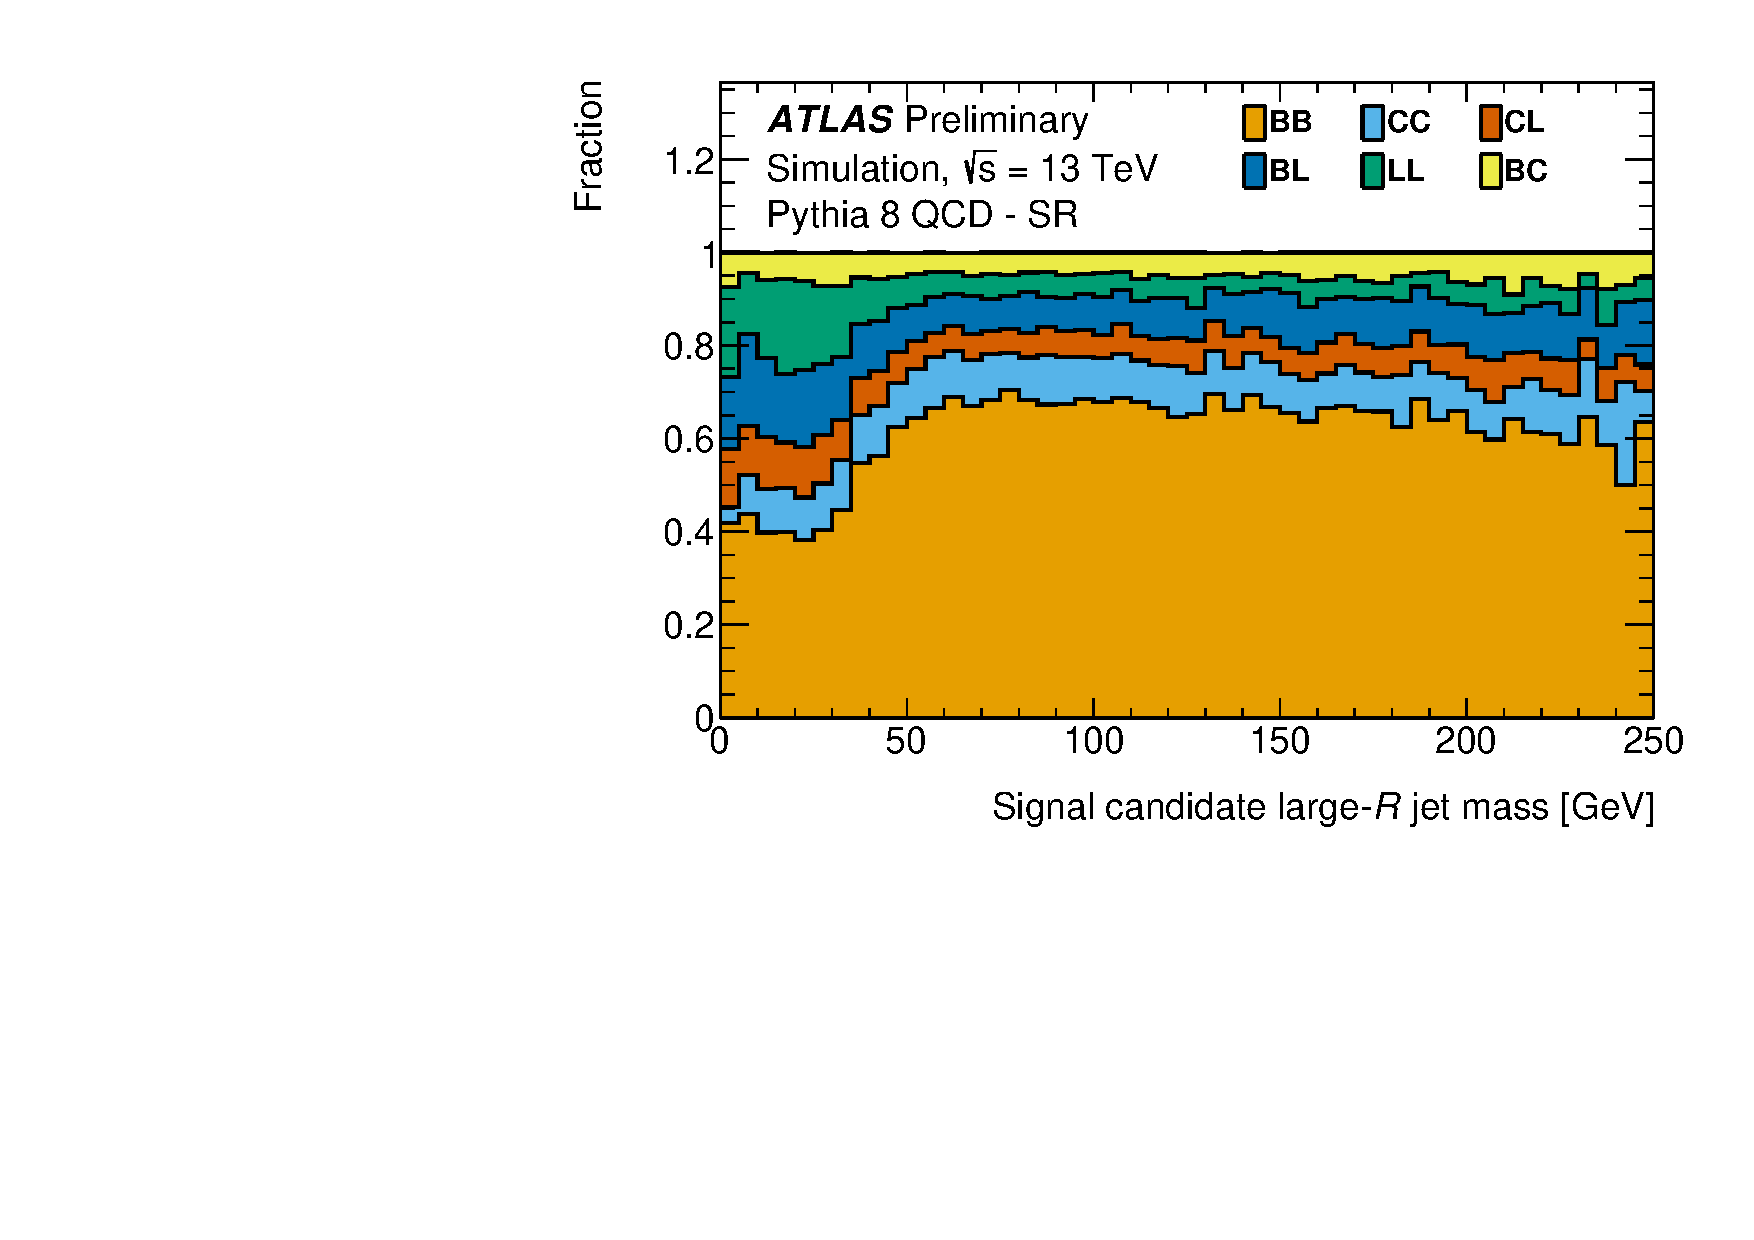
\includegraphics[width=0.48\textwidth]{figures/selection/flavor_composition}}\hfill
\subcaptionbox{\label{fig:selection:sr_cr_shape}}{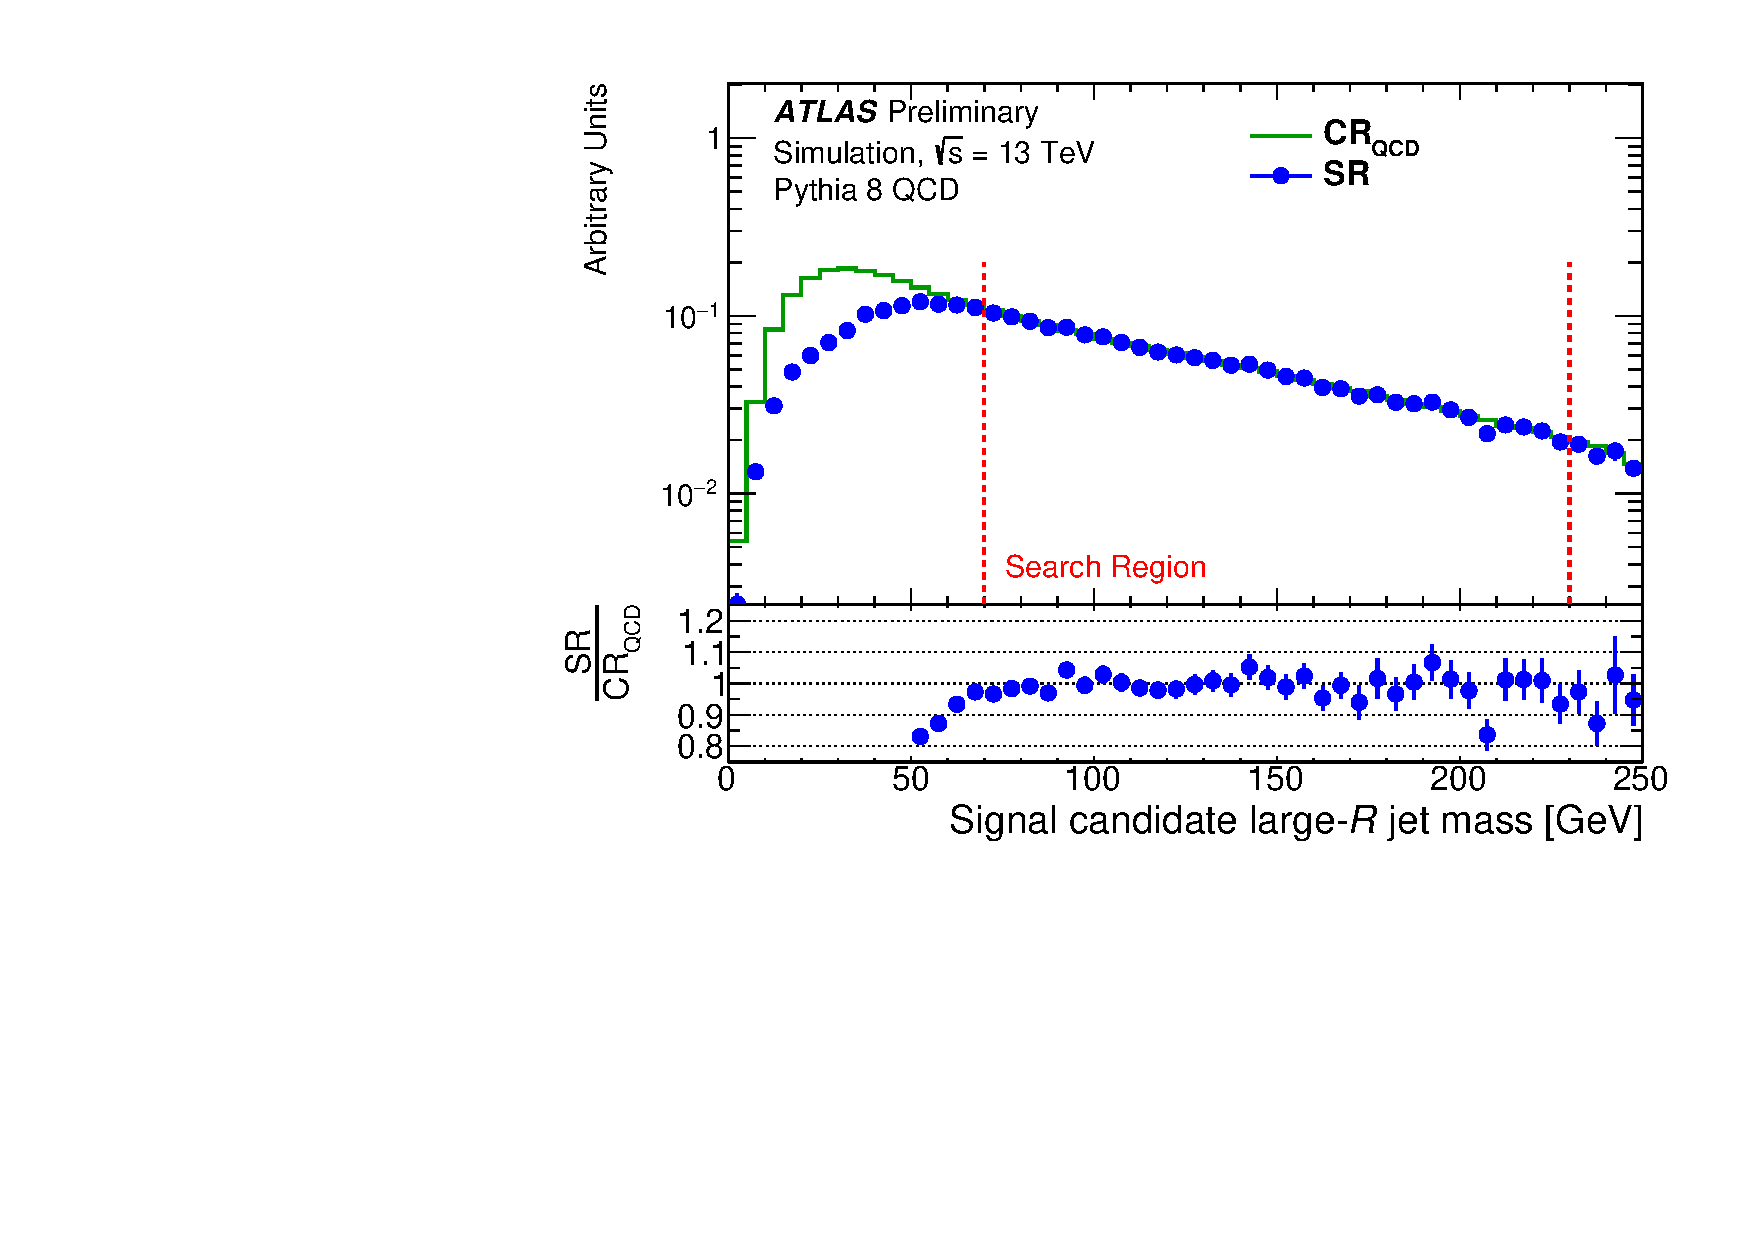
\includegraphics[width=0.48\textwidth]{figures/selection/sr_cr_shape}}

\caption{(a) Predicted flavor composition of the dijet background in the SR based on the truth-matched hadron content of the two leading-\pt track-jets associated to the signal candidate large-$R$ jet, with the B/C labels indicating the presence of a $b$/$c$-quark and L indicating the presence of a light quark or a gluon. (b) The expected shape of the dijet background in the SR and CR normalized to the same event count between $70~\GeV < m_{J} < 230~\GeV$ \cite{ATLAS-CONF-2018-052}.}
\label{fig:flavor_shape}
\end{figure}

\begin{table}[!htbp]
  \centering
  \begin{tabular}{l|l||c|c|c|c||c}
    & \textbf{Cut} & \textbf{ggF} & \textbf{VBF} & \textbf{WH} & \textbf{ZH} & \textbf{Total} \\
    \hline
    \hline
    \textbf{Preselection} & Trigger                                & \CutflowCRqcdGGFtrigger    & \CutflowCRqcdVBFtrigger    & \CutflowCRqcdWHtrigger    & \CutflowCRqcdZHtrigger    & \CutflowCRqcdHiggstrigger \\
                          & Jet Cleaning                           & \CutflowCRqcdGGFcleaning   & \CutflowCRqcdVBFcleaning   & \CutflowCRqcdWHcleaning   & \CutflowCRqcdZHcleaning   & \CutflowCRqcdHiggscleaning \\
                          & Lead \largeR jet \pt$>480~\GeV$        & \CutflowCRqcdGGFfatjetZero & \CutflowCRqcdVBFfatjetZero & \CutflowCRqcdWHfatjetZero & \CutflowCRqcdZHfatjetZero & \CutflowCRqcdHiggsfatjetZero \\
                          & Sublead \largeR jet \pt$>250~\GeV$     & \CutflowCRqcdGGFfatjetOne  & \CutflowCRqcdVBFfatjetOne  & \CutflowCRqcdWHfatjetOne  & \CutflowCRqcdZHfatjetOne  & \CutflowCRqcdHiggsfatjetOne \\
                          & At least one signal candidate          & \CutflowCRqcdGGFZprimeCand & \CutflowCRqcdVBFZprimeCand & \CutflowCRqcdWHZprimeCand & \CutflowCRqcdZHZprimeCand & \CutflowCRqcdHiggsZprimeCand \\
                          & No opposite muon ($\text{CR}_{t\bar{t}}$ veto)        & \CutflowCRqcdGGFNoTTbarMuon& \CutflowCRqcdVBFNoTTbarMuon& \CutflowCRqcdWHNoTTbarMuon& \CutflowCRqcdZHNoTTbarMuon& \CutflowCRqcdHiggsNoTTbarMuon \\
                          & signal candidate \pt$>480~\GeV$        & \CutflowCRqcdGGFhcandpt    & \CutflowCRqcdVBFhcandpt    & \CutflowCRqcdWHhcandpt    & \CutflowCRqcdZHhcandpt    & \CutflowCRqcdHiggshcandpt \\
                          & signal candidate mass$>40~\GeV$        & \CutflowCRqcdGGFhcandm     & \CutflowCRqcdVBFhcandm     & \CutflowCRqcdWHhcandm     & \CutflowCRqcdZHhcandm     & \CutflowCRqcdHiggshcandm \\
    \hline
    \textbf{$\text{CR}_{\text{QCD}}$}        & 0 b-tagged VR subjets (85\% WP)        & \CutflowCRqcdGGFNBTag      & \CutflowCRqcdVBFNBTag      & \CutflowCRqcdWHNBTag      & \CutflowCRqcdZHNBTag      & \CutflowCRqcdHiggsNBTag \\
    \hline
    \textbf{SR}           & 2 b-tagged VR subjets (77\% WP)        & \CutflowSRGGFNBTag         & \CutflowSRVBFNBTag         & \CutflowSRWHNBTag         & \CutflowSRZHNBTag         & \CutflowSRHiggsNBTag \\
  \end{tabular}
  \caption{Cutflow showing the effect in simulation of selection criteria for each of the Higgs boson production mechanisms \cite{Krizka:2310645}. The numbers here can be compared to the number of events generated as shown in \Cref{table:data:signal}.}
  \label{tab:selection:cutflow_higgs}
\end{table}

\begin{table}[!htbp]
\centerline{
  \centering
  {\footnotesize
  \begin{tabular}{l|l||c|c|c|c|c||c}
    & \textbf{Cut} & \textbf{QCD} & \textbf{W+jets} & \textbf{Z+jets} & $\boldsymbol{t\bar{t}}$ & \textbf{Total} & \textbf{Data} \\
    \hline
    \hline
    \textbf{Preselection} & Trigger                                & \CutflowCRqcdQCDtrigger    & \CutflowCRqcdWtrigger    & \CutflowCRqcdZtrigger    & \CutflowCRqcdTTbartrigger    & \CutflowCRqcdTotaltrigger    & \CutflowCRqcdDatatrigger \\
                          & Jet Cleaning                           & \CutflowCRqcdQCDcleaning   & \CutflowCRqcdWcleaning   & \CutflowCRqcdZcleaning   & \CutflowCRqcdTTbarcleaning   & \CutflowCRqcdTotalcleaning   & \CutflowCRqcdDatacleaning \\
                          & Lead \largeR jet \pt$>480~\GeV$        & \CutflowCRqcdQCDfatjetZero & \CutflowCRqcdWfatjetZero & \CutflowCRqcdZfatjetZero & \CutflowCRqcdTTbarfatjetZero & \CutflowCRqcdTotalfatjetZero & \CutflowCRqcdDatafatjetZero \\
                          & Sublead \largeR jet \pt$>250~\GeV$     & \CutflowCRqcdQCDfatjetOne  & \CutflowCRqcdWfatjetOne  & \CutflowCRqcdZfatjetOne  & \CutflowCRqcdTTbarfatjetOne  & \CutflowCRqcdTotalfatjetOne  & \CutflowCRqcdDatafatjetOne \\
                          & At least one signal candidate          & \CutflowCRqcdQCDZprimeCand & \CutflowCRqcdWZprimeCand & \CutflowCRqcdZZprimeCand & \CutflowCRqcdTTbarZprimeCand & \CutflowCRqcdTotalZprimeCand & \CutflowCRqcdDataZprimeCand \\
                          & No opposite muon ($\text{CR}_{t\bar{t}}$ veto)        & \CutflowCRqcdQCDNoTTbarMuon& \CutflowCRqcdWNoTTbarMuon& \CutflowCRqcdZNoTTbarMuon& \CutflowCRqcdTTbarNoTTbarMuon& \CutflowCRqcdTotalNoTTbarMuon& \CutflowCRqcdDataNoTTbarMuon \\
                          & signal candidate \pt$>480~\GeV$        & \CutflowCRqcdQCDhcandpt    & \CutflowCRqcdWhcandpt    & \CutflowCRqcdZhcandpt    & \CutflowCRqcdTTbarhcandpt    & \CutflowCRqcdTotalhcandpt    & \CutflowCRqcdDatahcandpt \\
                          & signal candidate mass$>40~\GeV$        & \CutflowCRqcdQCDhcandm     & \CutflowCRqcdWhcandm     & \CutflowCRqcdZhcandm     & \CutflowCRqcdTTbarhcandm     & \CutflowCRqcdTotalhcandm     & \CutflowCRqcdDatahcandm \\
    \hline
    \textbf{$\text{CR}_{\text{QCD}}$}        & 0 b-tagged VR subjets (85\% WP)        & \CutflowCRqcdQCDNBTag      & \CutflowCRqcdWNBTag      & \CutflowCRqcdZNBTag      & \CutflowCRqcdTTbarNBTag      & \CutflowCRqcdTotalNBTag      & \CutflowCRqcdDataNBTag \\
    \hline
    \textbf{SR}           & 2 b-tagged VR subjets (77\% WP)        & \CutflowSRQCDNBTag         & \CutflowSRWNBTag         & \CutflowSRZNBTag         & \CutflowSRTTbarNBTag         & \CutflowSRTotalNBTag         & \CutflowSRDataNBTag \\
  \end{tabular}}
}
  \caption{Cutflow showing the effect of selection criteria on simulated background samples as well as data. The simulated QCD contribution is scaled by $0.74$ which was derived from a fit to data in the $\text{CR}_{\text{QCD}}$ \cite{Krizka:2310645}. The background simulation numbers here can be compared to the number of events generated as shown in \Cref{table:data:QCD,table:data:V_hadronic,table:data:ttbar}.}
  \label{tab:selection:cutflow_bkg}
\end{table}

The QCD estimate is only valid for regions where the SR and
$\text{CR}_{\text{QCD}}$ have a similar dijet mass shape.  This results in a
lower bound cut on the signal candidate mass of $m_{J} > 70~\GeV$ due to the
higher turn-on curve of the SR shown in \Cref{fig:selection:sr_cr_shape}. This
low mass turn on is due to the $b$-tagging algorithm not being able to resolve
the $b$-jets as they begin to overlap.  Furthermore, for $m_{J} > 230~\GeV$ the
boost from a $\pT$ of $480~\GeV$ is no longer sufficient to merge two hadrons
into a single large-$R$ jet.  Thus the SR signal candidate masses considered in
the analysis range from $70~\GeV$ to $230~\GeV$.

Given the above criteria, the efficiencies and yields in the SR and
$\text{CR}_{\text{QCD}}$ for the resonant backgrounds and the Higgs boson
signal are shown in \Cref{table:efficiencies_and_yields}. The composition of
the  vector boson, $t\bar{t}$ and $H \rightarrow b\bar{b}$ resonant components
of the SR and $\text{CR}_{\text{QCD}}$ are given in
\Cref{table:fractional_composition}. For the vector boson background, the
$W+\text{jets}$ contribution dominates in the $\text{CR}_{\text{QCD}}$ due to
its larger cross section.  However, the $Z+\text{jets}$ dominates in the SR as
the $Z$ boson can decay to two $b$-quarks.  The $t\bar{t}$ contribution is
roughly the same in the SR and $\text{CR}_{\text{QCD}}$ with $\sim 60\%$ of
events decaying entirely to hadrons (all hadronic), $\sim 40\%$ of events with
one $W$ boson decaying leptonically (semi-leptonic), and a small percentage of
events with both $W$ bosons decaying leptonically (dileptonic). In the SR the
dominant $H \rightarrow b\bar{b}$ production mechanism is ggF, contributing
53\% of the signal, followed by VBF production with 25\% and Higgstrahlung at
22\%. 

\begin{table}[htpb]
 \centering
 \caption{The efficiencies and yields in the $0$-tag control region ($\text{CR}_{\text{QCD}}$) and signal region (SR) for the non-QCD background, the Higgs boson signal and data. The yields in the $\text{CR}_{\text{QCD}}$ are scaled to the luminosity used for the background estimate of the non-resonant dijet process discussed in \Cref{sec:background:qcd}. The efficiencies are calculated relative to the leading large-$R$ jet $\pT > 480~\GeV$ requirement \cite{Krizka:2310645}.}
 \begin{adjustbox}{max width=\textwidth}
  \begin{tabular}{@{}lrrrrr@{}}
   \toprule
   Process                             & $\text{CR}_{\text{QCD}}$ Eff. $(\%)$ & $\text{CR}_{\text{QCD}}$ Yield in $1.4~\ifb$ & SR Eff. $(\%)$ & SR Yield in $80.5~\ifb$ \\ \midrule
   $W \to q\bar{q} + \text{jets}$    & $51.3$               & $3810$                       & $0.4$          & $1500$                  \\
   $Z \to q\bar{q} + \text{jets}$    & $46.2$               & $1470$                       & $3.4$          & $6200$                  \\
   $t\bar{t}$                          & $25.9$               & $1929$                       & $2.5$          & $10550$                 \\
   $H \rightarrow b\bar{b}$                              & $24.3$               & $5$                          & $17.9$         & $216$                   \\
   \phantom{$H \rightarrow b\bar{b}$\quad}~ggF           & $23.6$               & $2$                          & $19.4$         & $115$                   \\
   \phantom{$H \rightarrow b\bar{b}$\quad}~VBF           & $15.8$               & $1$                          & $20.7$         & $53$                    \\
   \phantom{$H \rightarrow b\bar{b}$\quad}~$WH$          & $32.4$               & $1$                          & $12.0$         & $26$                    \\
   \phantom{$H \rightarrow b\bar{b}$\quad}~$ZH$          & $30.5$               & $1$                          & $15.8$         & $21$                    \\
   Data                                & $38.7$               & $519710$                     & $0.6$          & $484600$                \\
   \bottomrule
  \end{tabular}
 \end{adjustbox}
 \label{table:efficiencies_and_yields}
\end{table}

\begin{table}[htpb]
 \centering
 \caption{The fractional composition of the different resonant contributions in the $0$-tag control region ($\text{CR}_{\text{QCD}}$) and the signal region (SR). The fraction is evaluated using the given contribution type as the total \cite{Krizka:2310645}.}
 \begin{tabular}{@{}lrr@{}}
  \toprule
  Process                                   & $\text{CR}_{\text{QCD}}$ Fraction & SR Fraction \\ \midrule
  $V+\text{jets}$                                  &                   &             \\
  \phantom{$V+\text{jets}$\quad} $Z+\text{jets}$ & $0.28$            & $0.80$      \\
  \phantom{$V+\text{jets}$\quad} $W+\text{jets}$ & $0.72$            & $0.20$      \\
  $t\bar{t}$                                &                   &             \\
  \phantom{$t\bar{t}$\quad} hadronic        & $0.58$            & $0.63$      \\
  \phantom{$t\bar{t}$\quad} semi-leptonic   & $0.38$            & $0.34$      \\
  \phantom{$t\bar{t}$\quad} dileptonic      & $0.04$            & $0.03$      \\
  $H \rightarrow b\bar{b}$                                    &                   &             \\
  \phantom{$H \rightarrow b\bar{b}$\quad} ggF                 & $0.50$            & $0.53$      \\
  \phantom{$H \rightarrow b\bar{b}$\quad} VBF                 & $0.17$            & $0.25$      \\
  \phantom{$H \rightarrow b\bar{b}$\quad} $WH$                & $0.21$            & $0.12$      \\
  \phantom{$H \rightarrow b\bar{b}$\quad} $ZH$                & $0.12$            & $0.10$      \\
  \bottomrule
 \end{tabular}
 \label{table:fractional_composition}
\end{table}

